% Created by tikzDevice version 0.12.6 on 2025-02-04 13:53:24
% !TEX encoding = UTF-8 Unicode
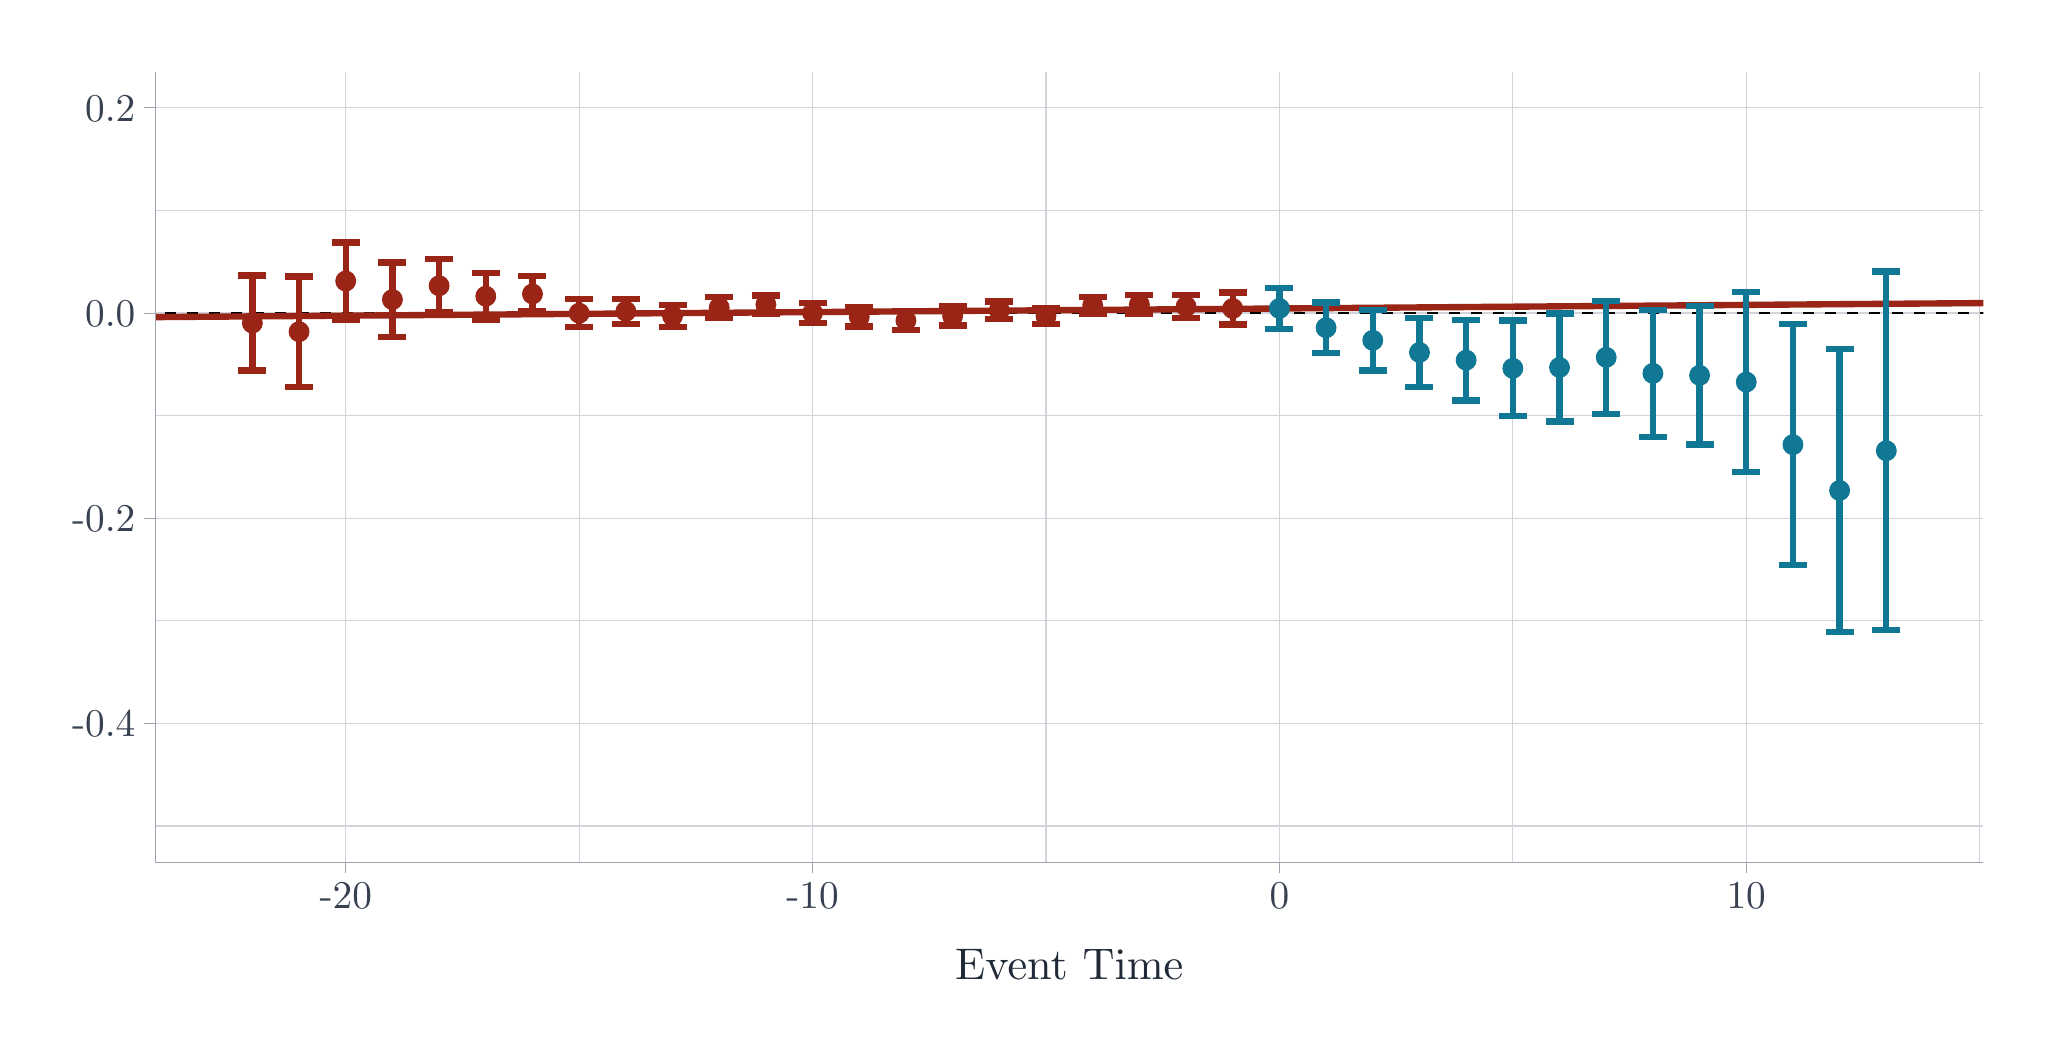
\begin{tikzpicture}[x=1pt,y=1pt]
\definecolor{fillColor}{RGB}{255,255,255}
\path[use as bounding box,fill=fillColor] (0,0) rectangle (722.70,361.35);
\begin{scope}
\path[clip] (  0.00,  0.00) rectangle (722.70,361.35);
\definecolor{drawColor}{RGB}{255,255,255}

\path[draw=drawColor,line width= 0.8pt,line join=round,line cap=round,fill=fillColor] (  0.00,  0.00) rectangle (722.70,361.35);
\end{scope}
\begin{scope}
\path[clip] ( 46.10, 59.89) rectangle (706.70,345.35);
\definecolor{drawColor}{RGB}{255,255,255}
\definecolor{fillColor}{RGB}{255,255,255}

\path[draw=drawColor,line width= 0.8pt,line join=round,line cap=round,fill=fillColor] ( 46.10, 59.89) rectangle (706.70,345.35);
\definecolor{drawColor}{RGB}{209,213,219}

\path[draw=drawColor,line width= 0.4pt,line join=round] ( 46.10, 72.86) --
	(706.70, 72.86);

\path[draw=drawColor,line width= 0.4pt,line join=round] ( 46.10,147.01) --
	(706.70,147.01);

\path[draw=drawColor,line width= 0.4pt,line join=round] ( 46.10,221.16) --
	(706.70,221.16);

\path[draw=drawColor,line width= 0.4pt,line join=round] ( 46.10,295.30) --
	(706.70,295.30);

\path[draw=drawColor,line width= 0.4pt,line join=round] (199.28, 59.89) --
	(199.28,345.35);

\path[draw=drawColor,line width= 0.4pt,line join=round] (367.97, 59.89) --
	(367.97,345.35);

\path[draw=drawColor,line width= 0.4pt,line join=round] (536.66, 59.89) --
	(536.66,345.35);

\path[draw=drawColor,line width= 0.4pt,line join=round] (705.35, 59.89) --
	(705.35,345.35);

\path[draw=drawColor,line width= 0.4pt,line join=round] ( 46.10,109.94) --
	(706.70,109.94);

\path[draw=drawColor,line width= 0.4pt,line join=round] ( 46.10,184.08) --
	(706.70,184.08);

\path[draw=drawColor,line width= 0.4pt,line join=round] ( 46.10,258.23) --
	(706.70,258.23);

\path[draw=drawColor,line width= 0.4pt,line join=round] ( 46.10,332.37) --
	(706.70,332.37);

\path[draw=drawColor,line width= 0.4pt,line join=round] (114.93, 59.89) --
	(114.93,345.35);

\path[draw=drawColor,line width= 0.4pt,line join=round] (283.62, 59.89) --
	(283.62,345.35);

\path[draw=drawColor,line width= 0.4pt,line join=round] (452.31, 59.89) --
	(452.31,345.35);

\path[draw=drawColor,line width= 0.4pt,line join=round] (621.00, 59.89) --
	(621.00,345.35);
\definecolor{drawColor}{RGB}{0,0,0}

\path[draw=drawColor,line width= 0.9pt,dash pattern=on 4pt off 4pt ,line join=round] (-614.49,258.23) -- (1367.30,258.23);
\definecolor{drawColor}{RGB}{154,36,21}

\path[draw=drawColor,line width= 2.3pt,line join=round] (-614.49,251.67) -- (1367.30,266.91);
\definecolor{fillColor}{RGB}{154,36,21}

\path[draw=drawColor,line width= 0.4pt,line join=round,line cap=round,fill=fillColor] ( 81.19,254.61) circle (  3.57);

\path[draw=drawColor,line width= 0.4pt,line join=round,line cap=round,fill=fillColor] ( 98.06,251.49) circle (  3.57);

\path[draw=drawColor,line width= 0.4pt,line join=round,line cap=round,fill=fillColor] (114.93,269.80) circle (  3.57);

\path[draw=drawColor,line width= 0.4pt,line join=round,line cap=round,fill=fillColor] (131.80,263.10) circle (  3.57);

\path[draw=drawColor,line width= 0.4pt,line join=round,line cap=round,fill=fillColor] (148.67,268.08) circle (  3.57);

\path[draw=drawColor,line width= 0.4pt,line join=round,line cap=round,fill=fillColor] (165.54,264.31) circle (  3.57);

\path[draw=drawColor,line width= 0.4pt,line join=round,line cap=round,fill=fillColor] (182.41,265.12) circle (  3.57);

\path[draw=drawColor,line width= 0.4pt,line join=round,line cap=round,fill=fillColor] (199.28,258.18) circle (  3.57);

\path[draw=drawColor,line width= 0.4pt,line join=round,line cap=round,fill=fillColor] (216.15,258.85) circle (  3.57);

\path[draw=drawColor,line width= 0.4pt,line join=round,line cap=round,fill=fillColor] (233.01,257.15) circle (  3.57);

\path[draw=drawColor,line width= 0.4pt,line join=round,line cap=round,fill=fillColor] (249.88,260.18) circle (  3.57);

\path[draw=drawColor,line width= 0.4pt,line join=round,line cap=round,fill=fillColor] (266.75,261.28) circle (  3.57);

\path[draw=drawColor,line width= 0.4pt,line join=round,line cap=round,fill=fillColor] (283.62,258.27) circle (  3.57);

\path[draw=drawColor,line width= 0.4pt,line join=round,line cap=round,fill=fillColor] (300.49,256.83) circle (  3.57);

\path[draw=drawColor,line width= 0.4pt,line join=round,line cap=round,fill=fillColor] (317.36,255.52) circle (  3.57);

\path[draw=drawColor,line width= 0.4pt,line join=round,line cap=round,fill=fillColor] (334.23,257.13) circle (  3.57);

\path[draw=drawColor,line width= 0.4pt,line join=round,line cap=round,fill=fillColor] (351.10,259.20) circle (  3.57);

\path[draw=drawColor,line width= 0.4pt,line join=round,line cap=round,fill=fillColor] (367.97,257.16) circle (  3.57);

\path[draw=drawColor,line width= 0.4pt,line join=round,line cap=round,fill=fillColor] (384.84,261.00) circle (  3.57);

\path[draw=drawColor,line width= 0.4pt,line join=round,line cap=round,fill=fillColor] (401.71,261.33) circle (  3.57);

\path[draw=drawColor,line width= 0.4pt,line join=round,line cap=round,fill=fillColor] (418.58,260.60) circle (  3.57);

\path[draw=drawColor,line width= 0.4pt,line join=round,line cap=round,fill=fillColor] (435.44,259.87) circle (  3.57);
\definecolor{drawColor}{RGB}{16,120,149}
\definecolor{fillColor}{RGB}{16,120,149}

\path[draw=drawColor,line width= 0.4pt,line join=round,line cap=round,fill=fillColor] (452.31,259.90) circle (  3.57);

\path[draw=drawColor,line width= 0.4pt,line join=round,line cap=round,fill=fillColor] (469.18,252.92) circle (  3.57);

\path[draw=drawColor,line width= 0.4pt,line join=round,line cap=round,fill=fillColor] (486.05,248.37) circle (  3.57);

\path[draw=drawColor,line width= 0.4pt,line join=round,line cap=round,fill=fillColor] (502.92,243.99) circle (  3.57);

\path[draw=drawColor,line width= 0.4pt,line join=round,line cap=round,fill=fillColor] (519.79,241.21) circle (  3.57);

\path[draw=drawColor,line width= 0.4pt,line join=round,line cap=round,fill=fillColor] (536.66,238.25) circle (  3.57);

\path[draw=drawColor,line width= 0.4pt,line join=round,line cap=round,fill=fillColor] (553.53,238.57) circle (  3.57);

\path[draw=drawColor,line width= 0.4pt,line join=round,line cap=round,fill=fillColor] (570.40,242.22) circle (  3.57);

\path[draw=drawColor,line width= 0.4pt,line join=round,line cap=round,fill=fillColor] (587.27,236.44) circle (  3.57);

\path[draw=drawColor,line width= 0.4pt,line join=round,line cap=round,fill=fillColor] (604.14,235.73) circle (  3.57);

\path[draw=drawColor,line width= 0.4pt,line join=round,line cap=round,fill=fillColor] (621.00,233.30) circle (  3.57);

\path[draw=drawColor,line width= 0.4pt,line join=round,line cap=round,fill=fillColor] (637.87,210.67) circle (  3.57);

\path[draw=drawColor,line width= 0.4pt,line join=round,line cap=round,fill=fillColor] (654.74,194.11) circle (  3.57);

\path[draw=drawColor,line width= 0.4pt,line join=round,line cap=round,fill=fillColor] (671.61,208.47) circle (  3.57);
\definecolor{drawColor}{RGB}{154,36,21}

\path[draw=drawColor,line width= 2.3pt,line join=round] ( 76.13,271.81) --
	( 86.25,271.81);

\path[draw=drawColor,line width= 2.3pt,line join=round] ( 81.19,271.81) --
	( 81.19,237.42);

\path[draw=drawColor,line width= 2.3pt,line join=round] ( 76.13,237.42) --
	( 86.25,237.42);

\path[draw=drawColor,line width= 2.3pt,line join=round] ( 93.00,271.44) --
	(103.12,271.44);

\path[draw=drawColor,line width= 2.3pt,line join=round] ( 98.06,271.44) --
	( 98.06,231.54);

\path[draw=drawColor,line width= 2.3pt,line join=round] ( 93.00,231.54) --
	(103.12,231.54);

\path[draw=drawColor,line width= 2.3pt,line join=round] (109.87,283.74) --
	(119.99,283.74);

\path[draw=drawColor,line width= 2.3pt,line join=round] (114.93,283.74) --
	(114.93,255.86);

\path[draw=drawColor,line width= 2.3pt,line join=round] (109.87,255.86) --
	(119.99,255.86);

\path[draw=drawColor,line width= 2.3pt,line join=round] (126.74,276.53) --
	(136.86,276.53);

\path[draw=drawColor,line width= 2.3pt,line join=round] (131.80,276.53) --
	(131.80,249.67);

\path[draw=drawColor,line width= 2.3pt,line join=round] (126.74,249.67) --
	(136.86,249.67);

\path[draw=drawColor,line width= 2.3pt,line join=round] (143.61,277.78) --
	(153.73,277.78);

\path[draw=drawColor,line width= 2.3pt,line join=round] (148.67,277.78) --
	(148.67,258.39);

\path[draw=drawColor,line width= 2.3pt,line join=round] (143.61,258.39) --
	(153.73,258.39);

\path[draw=drawColor,line width= 2.3pt,line join=round] (160.48,272.67) --
	(170.60,272.67);

\path[draw=drawColor,line width= 2.3pt,line join=round] (165.54,272.67) --
	(165.54,255.95);

\path[draw=drawColor,line width= 2.3pt,line join=round] (160.48,255.95) --
	(170.60,255.95);

\path[draw=drawColor,line width= 2.3pt,line join=round] (177.35,271.51) --
	(187.47,271.51);

\path[draw=drawColor,line width= 2.3pt,line join=round] (182.41,271.51) --
	(182.41,258.74);

\path[draw=drawColor,line width= 2.3pt,line join=round] (177.35,258.74) --
	(187.47,258.74);

\path[draw=drawColor,line width= 2.3pt,line join=round] (194.22,263.27) --
	(204.34,263.27);

\path[draw=drawColor,line width= 2.3pt,line join=round] (199.28,263.27) --
	(199.28,253.10);

\path[draw=drawColor,line width= 2.3pt,line join=round] (194.22,253.10) --
	(204.34,253.10);

\path[draw=drawColor,line width= 2.3pt,line join=round] (211.08,263.37) --
	(221.21,263.37);

\path[draw=drawColor,line width= 2.3pt,line join=round] (216.15,263.37) --
	(216.15,254.33);

\path[draw=drawColor,line width= 2.3pt,line join=round] (211.08,254.33) --
	(221.21,254.33);

\path[draw=drawColor,line width= 2.3pt,line join=round] (227.95,261.06) --
	(238.08,261.06);

\path[draw=drawColor,line width= 2.3pt,line join=round] (233.01,261.06) --
	(233.01,253.24);

\path[draw=drawColor,line width= 2.3pt,line join=round] (227.95,253.24) --
	(238.08,253.24);

\path[draw=drawColor,line width= 2.3pt,line join=round] (244.82,263.94) --
	(254.94,263.94);

\path[draw=drawColor,line width= 2.3pt,line join=round] (249.88,263.94) --
	(249.88,256.42);

\path[draw=drawColor,line width= 2.3pt,line join=round] (244.82,256.42) --
	(254.94,256.42);

\path[draw=drawColor,line width= 2.3pt,line join=round] (261.69,264.63) --
	(271.81,264.63);

\path[draw=drawColor,line width= 2.3pt,line join=round] (266.75,264.63) --
	(266.75,257.92);

\path[draw=drawColor,line width= 2.3pt,line join=round] (261.69,257.92) --
	(271.81,257.92);

\path[draw=drawColor,line width= 2.3pt,line join=round] (278.56,261.97) --
	(288.68,261.97);

\path[draw=drawColor,line width= 2.3pt,line join=round] (283.62,261.97) --
	(283.62,254.58);

\path[draw=drawColor,line width= 2.3pt,line join=round] (278.56,254.58) --
	(288.68,254.58);

\path[draw=drawColor,line width= 2.3pt,line join=round] (295.43,260.32) --
	(305.55,260.32);

\path[draw=drawColor,line width= 2.3pt,line join=round] (300.49,260.32) --
	(300.49,253.33);

\path[draw=drawColor,line width= 2.3pt,line join=round] (295.43,253.33) --
	(305.55,253.33);

\path[draw=drawColor,line width= 2.3pt,line join=round] (312.30,259.04) --
	(322.42,259.04);

\path[draw=drawColor,line width= 2.3pt,line join=round] (317.36,259.04) --
	(317.36,251.99);

\path[draw=drawColor,line width= 2.3pt,line join=round] (312.30,251.99) --
	(322.42,251.99);

\path[draw=drawColor,line width= 2.3pt,line join=round] (329.17,260.55) --
	(339.29,260.55);

\path[draw=drawColor,line width= 2.3pt,line join=round] (334.23,260.55) --
	(334.23,253.71);

\path[draw=drawColor,line width= 2.3pt,line join=round] (329.17,253.71) --
	(339.29,253.71);

\path[draw=drawColor,line width= 2.3pt,line join=round] (346.04,262.40) --
	(356.16,262.40);

\path[draw=drawColor,line width= 2.3pt,line join=round] (351.10,262.40) --
	(351.10,256.00);

\path[draw=drawColor,line width= 2.3pt,line join=round] (346.04,256.00) --
	(356.16,256.00);

\path[draw=drawColor,line width= 2.3pt,line join=round] (362.91,260.12) --
	(373.03,260.12);

\path[draw=drawColor,line width= 2.3pt,line join=round] (367.97,260.12) --
	(367.97,254.21);

\path[draw=drawColor,line width= 2.3pt,line join=round] (362.91,254.21) --
	(373.03,254.21);

\path[draw=drawColor,line width= 2.3pt,line join=round] (379.78,264.10) --
	(389.90,264.10);

\path[draw=drawColor,line width= 2.3pt,line join=round] (384.84,264.10) --
	(384.84,257.90);

\path[draw=drawColor,line width= 2.3pt,line join=round] (379.78,257.90) --
	(389.90,257.90);

\path[draw=drawColor,line width= 2.3pt,line join=round] (396.65,264.78) --
	(406.77,264.78);

\path[draw=drawColor,line width= 2.3pt,line join=round] (401.71,264.78) --
	(401.71,257.87);

\path[draw=drawColor,line width= 2.3pt,line join=round] (396.65,257.87) --
	(406.77,257.87);

\path[draw=drawColor,line width= 2.3pt,line join=round] (413.51,264.73) --
	(423.64,264.73);

\path[draw=drawColor,line width= 2.3pt,line join=round] (418.58,264.73) --
	(418.58,256.46);

\path[draw=drawColor,line width= 2.3pt,line join=round] (413.51,256.46) --
	(423.64,256.46);

\path[draw=drawColor,line width= 2.3pt,line join=round] (430.38,265.62) --
	(440.50,265.62);

\path[draw=drawColor,line width= 2.3pt,line join=round] (435.44,265.62) --
	(435.44,254.13);

\path[draw=drawColor,line width= 2.3pt,line join=round] (430.38,254.13) --
	(440.50,254.13);
\definecolor{drawColor}{RGB}{16,120,149}

\path[draw=drawColor,line width= 2.3pt,line join=round] (447.25,267.24) --
	(457.37,267.24);

\path[draw=drawColor,line width= 2.3pt,line join=round] (452.31,267.24) --
	(452.31,252.56);

\path[draw=drawColor,line width= 2.3pt,line join=round] (447.25,252.56) --
	(457.37,252.56);

\path[draw=drawColor,line width= 2.3pt,line join=round] (464.12,262.05) --
	(474.24,262.05);

\path[draw=drawColor,line width= 2.3pt,line join=round] (469.18,262.05) --
	(469.18,243.79);

\path[draw=drawColor,line width= 2.3pt,line join=round] (464.12,243.79) --
	(474.24,243.79);

\path[draw=drawColor,line width= 2.3pt,line join=round] (480.99,259.22) --
	(491.11,259.22);

\path[draw=drawColor,line width= 2.3pt,line join=round] (486.05,259.22) --
	(486.05,237.52);

\path[draw=drawColor,line width= 2.3pt,line join=round] (480.99,237.52) --
	(491.11,237.52);

\path[draw=drawColor,line width= 2.3pt,line join=round] (497.86,256.54) --
	(507.98,256.54);

\path[draw=drawColor,line width= 2.3pt,line join=round] (502.92,256.54) --
	(502.92,231.44);

\path[draw=drawColor,line width= 2.3pt,line join=round] (497.86,231.44) --
	(507.98,231.44);

\path[draw=drawColor,line width= 2.3pt,line join=round] (514.73,255.77) --
	(524.85,255.77);

\path[draw=drawColor,line width= 2.3pt,line join=round] (519.79,255.77) --
	(519.79,226.65);

\path[draw=drawColor,line width= 2.3pt,line join=round] (514.73,226.65) --
	(524.85,226.65);

\path[draw=drawColor,line width= 2.3pt,line join=round] (531.60,255.51) --
	(541.72,255.51);

\path[draw=drawColor,line width= 2.3pt,line join=round] (536.66,255.51) --
	(536.66,220.98);

\path[draw=drawColor,line width= 2.3pt,line join=round] (531.60,220.98) --
	(541.72,220.98);

\path[draw=drawColor,line width= 2.3pt,line join=round] (548.47,258.04) --
	(558.59,258.04);

\path[draw=drawColor,line width= 2.3pt,line join=round] (553.53,258.04) --
	(553.53,219.10);

\path[draw=drawColor,line width= 2.3pt,line join=round] (548.47,219.10) --
	(558.59,219.10);

\path[draw=drawColor,line width= 2.3pt,line join=round] (565.34,262.62) --
	(575.46,262.62);

\path[draw=drawColor,line width= 2.3pt,line join=round] (570.40,262.62) --
	(570.40,221.83);

\path[draw=drawColor,line width= 2.3pt,line join=round] (565.34,221.83) --
	(575.46,221.83);

\path[draw=drawColor,line width= 2.3pt,line join=round] (582.21,259.38) --
	(592.33,259.38);

\path[draw=drawColor,line width= 2.3pt,line join=round] (587.27,259.38) --
	(587.27,213.51);

\path[draw=drawColor,line width= 2.3pt,line join=round] (582.21,213.51) --
	(592.33,213.51);

\path[draw=drawColor,line width= 2.3pt,line join=round] (599.07,260.72) --
	(609.20,260.72);

\path[draw=drawColor,line width= 2.3pt,line join=round] (604.14,260.72) --
	(604.14,210.74);

\path[draw=drawColor,line width= 2.3pt,line join=round] (599.07,210.74) --
	(609.20,210.74);

\path[draw=drawColor,line width= 2.3pt,line join=round] (615.94,265.80) --
	(626.07,265.80);

\path[draw=drawColor,line width= 2.3pt,line join=round] (621.00,265.80) --
	(621.00,200.80);

\path[draw=drawColor,line width= 2.3pt,line join=round] (615.94,200.80) --
	(626.07,200.80);

\path[draw=drawColor,line width= 2.3pt,line join=round] (632.81,254.19) --
	(642.93,254.19);

\path[draw=drawColor,line width= 2.3pt,line join=round] (637.87,254.19) --
	(637.87,167.15);

\path[draw=drawColor,line width= 2.3pt,line join=round] (632.81,167.15) --
	(642.93,167.15);

\path[draw=drawColor,line width= 2.3pt,line join=round] (649.68,245.34) --
	(659.80,245.34);

\path[draw=drawColor,line width= 2.3pt,line join=round] (654.74,245.34) --
	(654.74,142.87);

\path[draw=drawColor,line width= 2.3pt,line join=round] (649.68,142.87) --
	(659.80,142.87);

\path[draw=drawColor,line width= 2.3pt,line join=round] (666.55,273.24) --
	(676.67,273.24);

\path[draw=drawColor,line width= 2.3pt,line join=round] (671.61,273.24) --
	(671.61,143.69);

\path[draw=drawColor,line width= 2.3pt,line join=round] (666.55,143.69) --
	(676.67,143.69);
\end{scope}
\begin{scope}
\path[clip] (  0.00,  0.00) rectangle (722.70,361.35);
\definecolor{drawColor}{RGB}{156,163,175}

\path[draw=drawColor,line width= 0.3pt,line join=round] ( 46.10, 59.89) --
	( 46.10,345.35);
\end{scope}
\begin{scope}
\path[clip] (  0.00,  0.00) rectangle (722.70,361.35);
\definecolor{drawColor}{RGB}{55,65,81}

\node[text=drawColor,anchor=base east,inner sep=0pt, outer sep=0pt, scale=  1.42] at ( 38.90,105.04) {-0.4};

\node[text=drawColor,anchor=base east,inner sep=0pt, outer sep=0pt, scale=  1.42] at ( 38.90,179.19) {-0.2};

\node[text=drawColor,anchor=base east,inner sep=0pt, outer sep=0pt, scale=  1.42] at ( 38.90,253.33) {0.0};

\node[text=drawColor,anchor=base east,inner sep=0pt, outer sep=0pt, scale=  1.42] at ( 38.90,327.48) {0.2};
\end{scope}
\begin{scope}
\path[clip] (  0.00,  0.00) rectangle (722.70,361.35);
\definecolor{drawColor}{RGB}{156,163,175}

\path[draw=drawColor,line width= 0.3pt,line join=round] ( 42.10,109.94) --
	( 46.10,109.94);

\path[draw=drawColor,line width= 0.3pt,line join=round] ( 42.10,184.08) --
	( 46.10,184.08);

\path[draw=drawColor,line width= 0.3pt,line join=round] ( 42.10,258.23) --
	( 46.10,258.23);

\path[draw=drawColor,line width= 0.3pt,line join=round] ( 42.10,332.37) --
	( 46.10,332.37);
\end{scope}
\begin{scope}
\path[clip] (  0.00,  0.00) rectangle (722.70,361.35);
\definecolor{drawColor}{RGB}{156,163,175}

\path[draw=drawColor,line width= 0.3pt,line join=round] ( 46.10, 59.89) --
	(706.70, 59.89);
\end{scope}
\begin{scope}
\path[clip] (  0.00,  0.00) rectangle (722.70,361.35);
\definecolor{drawColor}{RGB}{156,163,175}

\path[draw=drawColor,line width= 0.3pt,line join=round] (114.93, 55.89) --
	(114.93, 59.89);

\path[draw=drawColor,line width= 0.3pt,line join=round] (283.62, 55.89) --
	(283.62, 59.89);

\path[draw=drawColor,line width= 0.3pt,line join=round] (452.31, 55.89) --
	(452.31, 59.89);

\path[draw=drawColor,line width= 0.3pt,line join=round] (621.00, 55.89) --
	(621.00, 59.89);
\end{scope}
\begin{scope}
\path[clip] (  0.00,  0.00) rectangle (722.70,361.35);
\definecolor{drawColor}{RGB}{55,65,81}

\node[text=drawColor,anchor=base,inner sep=0pt, outer sep=0pt, scale=  1.42] at (114.93, 42.89) {-20};

\node[text=drawColor,anchor=base,inner sep=0pt, outer sep=0pt, scale=  1.42] at (283.62, 42.89) {-10};

\node[text=drawColor,anchor=base,inner sep=0pt, outer sep=0pt, scale=  1.42] at (452.31, 42.89) {0};

\node[text=drawColor,anchor=base,inner sep=0pt, outer sep=0pt, scale=  1.42] at (621.00, 42.89) {10};
\end{scope}
\begin{scope}
\path[clip] (  0.00,  0.00) rectangle (722.70,361.35);
\definecolor{drawColor}{RGB}{31,41,55}

\node[text=drawColor,anchor=base,inner sep=0pt, outer sep=0pt, scale=  1.60] at (376.40, 17.56) {Event Time};
\end{scope}
\end{tikzpicture}
